\documentclass[a4paper,10pt]{article}
\usepackage[utf8]{inputenc}
\usepackage{hyperref}
\usepackage{graphicx}
\usepackage{amssymb}
\usepackage{amsmath}
\usepackage[margin=0.7in]{geometry}

\title{Building a Granular Dataset of UK Companies}
\author{Alfred Holmes}


\date{September 2018}
\begin{document}
   \maketitle
   \begin{abstract}
   The UK government, through the Office for National Statistics and Companies House release detailed data on UK companies. Using this publicly available data, it is possible to track the location and assets of companies through time and using few assumptions assign branches, employees and turnover to these companies in such a way as to match the Office for National Statistics annual reports. This report summaries the available data and details the use of the data to compile a granular dataset.
   \end{abstract}
   \section{Introduction}
   To use contemporary techniques to model the UK economy, a detailed granular dataset of UK companies is required. Ideally the dataset would contain the employment size and turnover evolution of each company, as well as the location and number of employees of individual branches through time. From this, one could easily generate a detailed picture of the UK economy through time.
   \subsection{Definitions}
   These definitions are used consistently throughout this document, and provide clarity when describing subtly different entities.
   \begin{itemize}
 	\item Company - an entity registered on Companies House. In June 2017 there were 3.1 million registered companies in the UK. 
 	\item Enterprise - a business that is reported by ONS. We assume that an enterprise is a collection of companies. In 2017 the ONS reported 2.7 million enterprises.
 	\item Local Unit - a site where an enterprise operates, e.g. a branch of a large supermarket chain or the only location from which a small firm operates.
 	\item Local Authority - a connected area of land the UK governed by a council. At the time of writing, local authorities have a population of 170 000 people and 7 000 enterprises on average. There are 391 local authorities in the UK.
   \end{itemize}

   \section{Available Data}
   The UK government through Companies House and the Office for National statistics release detailed data. All data used in this study is provided through the Open Government License.
   \subsection{Companies House}
   Companies House is the public service responsible for incorporating and dissolving companies in the UK, as well as storing and releasing company data. They provide monthly snapshots of basic company information - names, registered office addresses, SIC codes - as well as all the online accounts that have been filed since 2008 and also provide an API where more detailed information - changes of address and people of significant control - can be accessed on a company by company basis.
   \subsubsection{Snapshots}
   The companies house snapshots \cite{companieshousesnapshots} are only available for the current month and only contain active companies and don't contain data on the history of each company. Luckily webarchive \cite{snapshotarchive} has archived approximately 1 snapshot per year, so this can be used to get low resolution historic data for companies. 
   \subsubsection{Accounts}
   If a company files its accounts online then that account filing is available to download through the companies house accounts data product \cite{accountsdataproduct}. This means that for increasingly many companies detailed financial data is available.
   The files are given as one XML (or HTML) file per account file per company per year. The most effective way to read these files is to recursively see if there is a number between two tags and if there is pull the number, its title and date. The \texttt{data/accounts} folder in the GitHub repository \cite{github} contains useful python scripts to process the accounts data. The following table summarises the available accounts data. The percentages proportion of accounts that contain the heading. There is a high correlation between having one of the heading and having the other. The proportion of filed accounts of active companies to active companies increases from 35\% in 2008 to about 60\% in 2017.
   \begin{center}
      \begin{tabular}{  l | c | c | c  }
      Year & Number of Accounts & netcurrentassetsliabilities & currentassets \\
      \hline
      2008 & 185163  & 59\% & 58\% \\
      2009 & 344403  & 64\% & 63\% \\
      2010 & 585143  & 71\% & 70\% \\
      2011 & 793218  & 74\% & 73\% \\
      2012 & 1033277 & 76\% & 74\% \\
      2013 & 1219357 & 77\% & 71\% \\
      2014 & 1573870 & 77\% & 72\% \\
      2015 & 1811446 & 77\% & 72\% \\
      2016 & 2071697 & 78\% & 72\% \\
      2017 & 2324272 & 79\% & 73\% \\

      \end{tabular}
   \end{center}


   \subsubsection{Companies House API}
   The Companies House API \cite{companieshouseapi} can be used to get detailed information about a company given its name or company number. The API has a request limit of 2 requests per second per API key, so to make one query per company for all companies registered since 2012 it would take 32 days. The service does allow multiple API keys to be registered which can speed up data acquisition. The API can be used to get all the filings for a particular company, with the exact dates of each. See the folder \texttt{data/API} in \cite{github} for a script that pulls the changes of address for companies.
   \subsection{Office for National Statistics}
   The Office for National Statistics releases yearly summery datasets
   \subsubsection{Business Activity, Size and Location}
   \label{basl}
   The Business Activity, Size and Location tables from the ONS \cite{basl}, available for 2012 to 2017, report by local authority and SIC code the number of companies with size in a particular range. For example, for employment statistics the ONS typically give the number of companies with employees in the ranges \emph{0-4, 5-9, 10-19, 20-49, 50-99, 100-249} and \emph{250+} and will do something similar for turnover.
   
   \subsubsection{Postcode Data}

   Since the data by location in \ref{basl} is by local authority, a useful resource is the postcode lookup tables \cite{postcodes}. These tables allow addresses of individual companies to be matched to local authorities. Included in the folder \texttt{useful} in \cite{github} is a slimmed down postcode table with just the postcode and its associated local authority's id as well as \texttt{lad\_17\_geo\_info.csv} which is a collection of the possible names on ONS documents and region information for each local authority\footnote{Local authority names sometimes have different spellings / word orders in different ONS datasets}.

   \subsubsection{Employment}

   The ONS also report employment \cite{employment} by location broken down into public and private sector jobs. We assume that all the companies listed on companies house are private entities, and hence any employees are working in the private sector.

   \section{Issues Combining ONS and Companies House data}


   \subsection{Number of Companies}
   \begin{figure}[h]
      \begin{center}
         \caption{Total Number of Companies registered on Companies House and reported by ONS}
         \label{ch_vs_ons}
         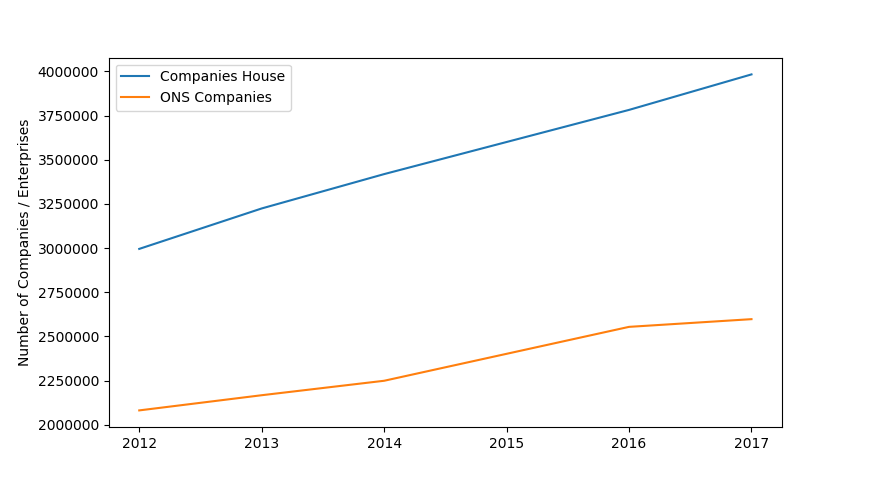
\includegraphics[width=12cm]{graphs/companies_house_vs_ons/companies_house_vs_ons}
      \end{center}
   \end{figure}
   % TODO: Removing repeated addresses for offices

   Looking at figure \ref{ch_vs_ons} it is clear that an ONS enterprise isn't just a companies house company. This is because many enterprises are made up of multiple companies. A way round this is to assume that if two companies have the same set of addresses then they are part of the same enterprise.

   \subsection{SIC Codes}

   Companies House companies can have multiple SIC codes and also have 5 digit SIC codes. The ONS release reports contain the number or enterprises with a particular 4 or 2 digit SIC code. It is not clear how they decide which SIC code to give to a particular enterprise, but it it likely that the enterprise give the SIC code in response to a survey so it would be difficult to infer the SIC code from an enterprise's companies as from the data it is difficult to work out the main business of an enterprise made up of many companies, each with multiple SIC codes. For this reason, the 4 digit SIC code data given by ONS does not match the companies house companies very well, but the 2 digit SIC codes match reasonably well. The 2 digit SIC codes are better because if a company reports two SIC codes, then it is likely that are in the same broad industry group and so they share the first two digits.

   \section{Fitting Lognormal Distributions}
   To make the ONS data usable some sort of size distribution needs to be assumed. This is not ideal since there are many different factors going in to company growth that can't be captured by simple growth models. Using Maximum Likelihood Estimation (MLE) and the ONS size bins as well as the mean company sizes, it is possible to fit distributions to the data. This has two benefits in that it assigns the mass of the probability distribution in a band in a sensible way and also removes the irritating \emph{250+} size band.
   
   \subsection{MLE}
  
   Assuming a lognormal distribution where the size X of a company is such that $\log X \sim \mathcal{N}(\mu, \sigma^2)$, $\mu$ and $\sigma$ can be estimated by maximising the log likelihood, given by
   \begin{equation}
   l(\mu, \sigma) = \sum_i n_i \log \left( \Phi \left( \frac{\log a_{i + 1} - \mu}{\sigma} \right) - \Phi \left( \frac{\log a_{i} - \mu}{\sigma} \right) \right)
   \end{equation}
   since $\mathbb{P}(a_i < X < a_{i + 1}) = \mathbb{P}(\log a_i < \log X < \log a_{i + 1}) = \Phi \left( \frac{\log a_{i + 1} - \mu}{\sigma} \right) - \Phi \left( \frac{\log a_{i} - \mu}{\sigma} \right)$. \\
   This parameter estimation is limited because the data is binned, and running experiments with we find that there is an error or bias with the recovered parameters that varies with the distribution parameters. For local authority and country wide parameter fitting, the total private employment, $e$, is released by ONS. From this, as the number of companies, $n$, is known the mean of the distribution can be used to constrain the parameters such that $\mu$ and $\sigma$ satisfy the equation $\exp(\mu + \sigma^2) = \frac{e}{n}$ in order to reduce the error of the predictions.

   \subsubsection{Simulations}

   In order to test whether the MLE can recover the distribution parameters from the size bins we ran simulations: picking random numbers from a known distribution and then trying to recover the distribution parameters. For these simulations we assume that the number of companies is large enough that the number of companies in each bin is the expected number of companies. The python scripts for these simulations can be found in the \texttt{Lognormal Bias} folder in \cite{github}. Running the script \texttt{analysis.py} gives an interactive version of the 3D graphs in figure \ref{bias}.


   \begin{figure}[!ht]
      \begin{center}
         \caption{Simulated Bias}
         \label{bias}
         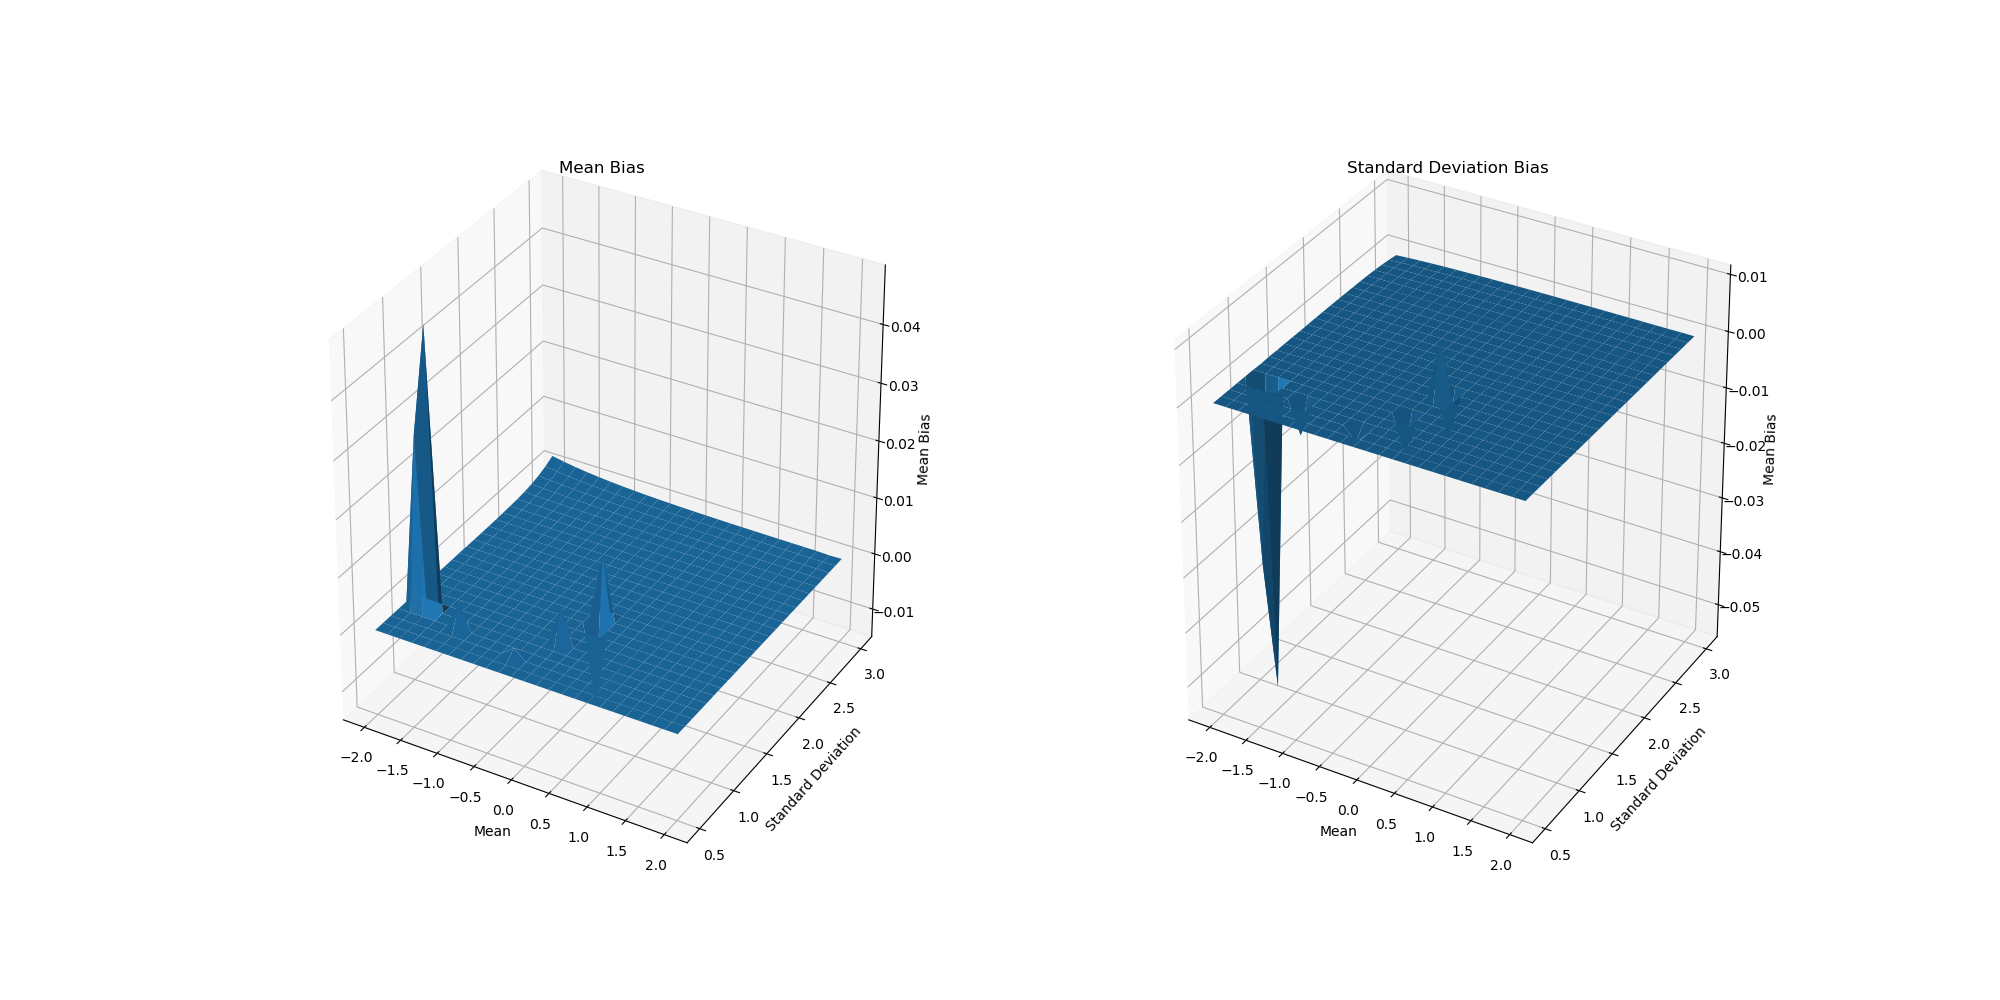
\includegraphics[width=\textwidth]{graphs/bias}
      \end{center}
   \end{figure}
   Figure \ref{bias} shows that the parameter estimation generally works quite well for the values 
   \subsubsection{Matching Enterprise Employment}
   \label{enterprise_employment}
   \section{Assigning Sizes and Turnover to companies}
   For this section we will focus on the year 2014. The same approach can be used for all the other years in the sample. To assign the size to companies we assume the following:
   \begin{itemize}
      \item Companies who do not report their assets have a small number of assets and have 0 or 1 employees.
      \item If company $a$ has more assets than company $b$ then company $a$ employs more people and company $b$. This could be refined such that this is only true for two companies with the same SIC code, but this adds complexity to the size assignments.
   \end{itemize}

   We then pull $n$ numbers from the fitted lognormal national distribution of company sizes, where $n$ is the total number of companies, and sort the list. We then sort the companies by asset size and assign company $i$ size $i$.
   Then plotting the results on a graph in a similar way to \ref{enterprise_employment} we get figure \ref{enterprise_employment_reconstruction}

   \begin{figure}
      \begin{center}
         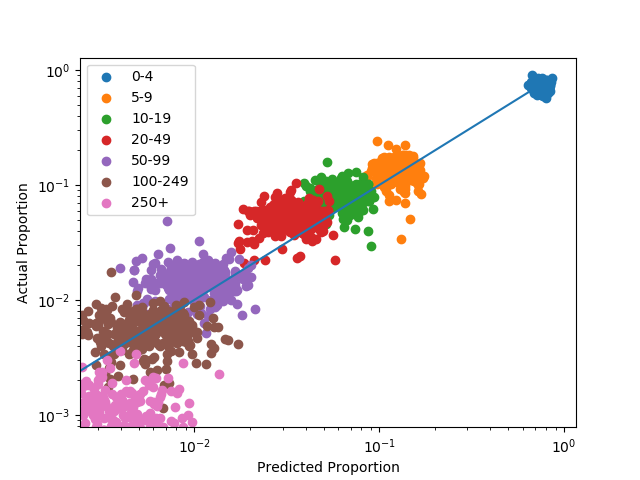
\includegraphics[width=10cm]{graphs/national_distribution_employment_reconstuction}
         \caption{National Employment Reconstruction}
         \label{enterprise_employment_reconstruction}
      \end{center}
   \end{figure}

   \subsection{Results}

   \medskip


   \begin{thebibliography}{9}
      \bibitem{companieshousesnapshots}
      Companies House Snapshot: list of basic company information for the current month's UK registered active companies
      \\\texttt{http://download.companieshouse.gov.uk/en\_output.html}

      \bibitem{snapshotarchive}Companies House Snapshot Archive
      \\\texttt{https://web.archive.org/web/20120901000000*/http://download.companieshouse.gov.uk/en\_output.html}

      \bibitem{accountsdataproduct}
      Accounts Data Product
      \\\texttt{http://download.companieshouse.gov.uk/historicmonthlyaccountsdata.html}
      
      \bibitem{github}
      UK Company Data GitHub repository
      \\\texttt{http://github.com/alfredholmes/uk-company-data}

      \bibitem{companieshouseapi} 
      Companies House API
      \\\texttt{https://developer.companieshouse.gov.uk/api/docs/}

      \bibitem{basl}
      Business Activity Size and Location
      \\2012:
      \\\texttt{http://webarchive.nationalarchives.gov.uk/20140511113648/http://www.ons.gov.uk/ons/publications/\\re-reference-tables.html?edition=tcm\%3A77-254601\&format=hi-vis}
      \\2013:
      \\\texttt{http://webarchive.nationalarchives.gov.uk/20140510023623/http://www.ons.gov.uk/ons/publications/\\re-reference-tables.html?edition=tcm\%3A77-313744\&format=hi-vis}
      \\2014 - 2017:
      \\\texttt{https://www.ons.gov.uk/businessindustryandtrade/business/activitysizeandlocation/datasets/\\ukbusinessactivitysizeandlocation}
      
      
      \bibitem{employment}
      ONS Employment Statistics
      \\\texttt{https://www.ons.gov.uk/employmentandlabourmarket/peopleinwork/employmentandemployeetypes/\\datasets/summaryoflabourmarketstatistics/current}

      \bibitem{postcodes}
      ONS Postcode Data
      \\\texttt{http://geoportal.statistics.gov.uk/datasets/postcode-to-output-area-to-lower-layer-super-output\\-area-to-middle-layer-super-output-area-to-local-authority-district-august-2018-lookup-in-the-uk}

   \end{thebibliography}








\end{document}